\documentclass{article}
\usepackage{ctex}
\usepackage{graphicx}
\usepackage{subfigure}
\usepackage{float}
\usepackage[a4paper,left=2cm,right=2cm,top=2cm,bottom=2cm]{geometry}
\usepackage{pythonhighlight}

\title{最大割问题优化算法课程报告}
\author{管实1801班~李博骁~U201815984\\管实1801班~李佳妮~U201816007\\管实1801班~李欣羽~U201816041}

\begin{document}
    \maketitle
    \newpage
    \tableofcontents
    \newpage

    \section{问题描述}
    最大割问题(Max-cut Problem),即对一个给定的图求一个最大分割,将所有顶点分为两群,使得被切断的边的边权之和最大,是图论中一个典型的NP-hard组合优化问题。

    其数学描述如下:
    给定无向图$G=(V,E)$,其中,$V=\{1,2,\dots,n\}$是所有顶点的集合;$E\subset V \times V$是所有边的集合;$w_{i,j}$为连接顶点$i,j$的边上的权。

    对于顶点集$V$的任一真子集$S$,令:
    \begin{equation}
        \delta(S)=\{e_{i,j}\in E;i\in S,j\in V-S\}
    \end{equation}

    即$\delta(S)$为边的集合,边的两端分别属于$S,V-S$,则由$S$确定的割$cut(S)$为:
    \begin{equation}
        cut(S)=\sum_{e_{i,j}\in \delta(S)} w_{i,j}
    \end{equation}

    最大割问题即找一个集合$S$,使得$cut(S)$最大。在本次作业中,给定的图为无权图,因而问题简化为使得$\delta(S)$中包含的边数最大。

    \section{算法描述与结果分析}
    此次作业中,我们小组使用Python实现了上课介绍的三种算法,并对这三种算法进行了相应的测试:
    \begin{itemize}
        \item 禁忌搜索算法(Tabu Search)
        \item 模拟退火算法(Simulated Annealing,SA)
        \item 遗传算法(Genetic Algorithm,GA)
    \end{itemize}
    
    算法对应代码文件分别见tabu\_search.py、simulated\_annealing.py与genetic\_algorithm.py。

    此外,根据要求,我们导出了记录迭代过程中解和目标值的变化情况的txt文件,并绘制了相应的目标值随迭代次数变化的图表,相应代码见plot\_data.py。

    \subsection{禁忌搜索算法}
    禁忌长度的设置考虑取节点数乘以一个可以自定义的乘数,即:
    \begin{equation}
        \mbox{禁忌长度} = \mbox{节点数} \times \mbox{禁忌长度乘数}
    \end{equation}

    最大迭代次数设定为5000,且给出的禁忌搜索算法中附加考虑了破禁准则,其具体运行机制如下:当被禁忌的邻域解中存在优于迄今为止所得最优解的解时,直接选择该解,在更新禁忌表后跳转下一步。

    随机选择一个禁忌长度(取禁忌长度乘数为0.05,即禁忌长度为6)进行测试得到迭代过程中目标值与最优目标值的变化如下:
    \begin{figure}[H]
        \centering
        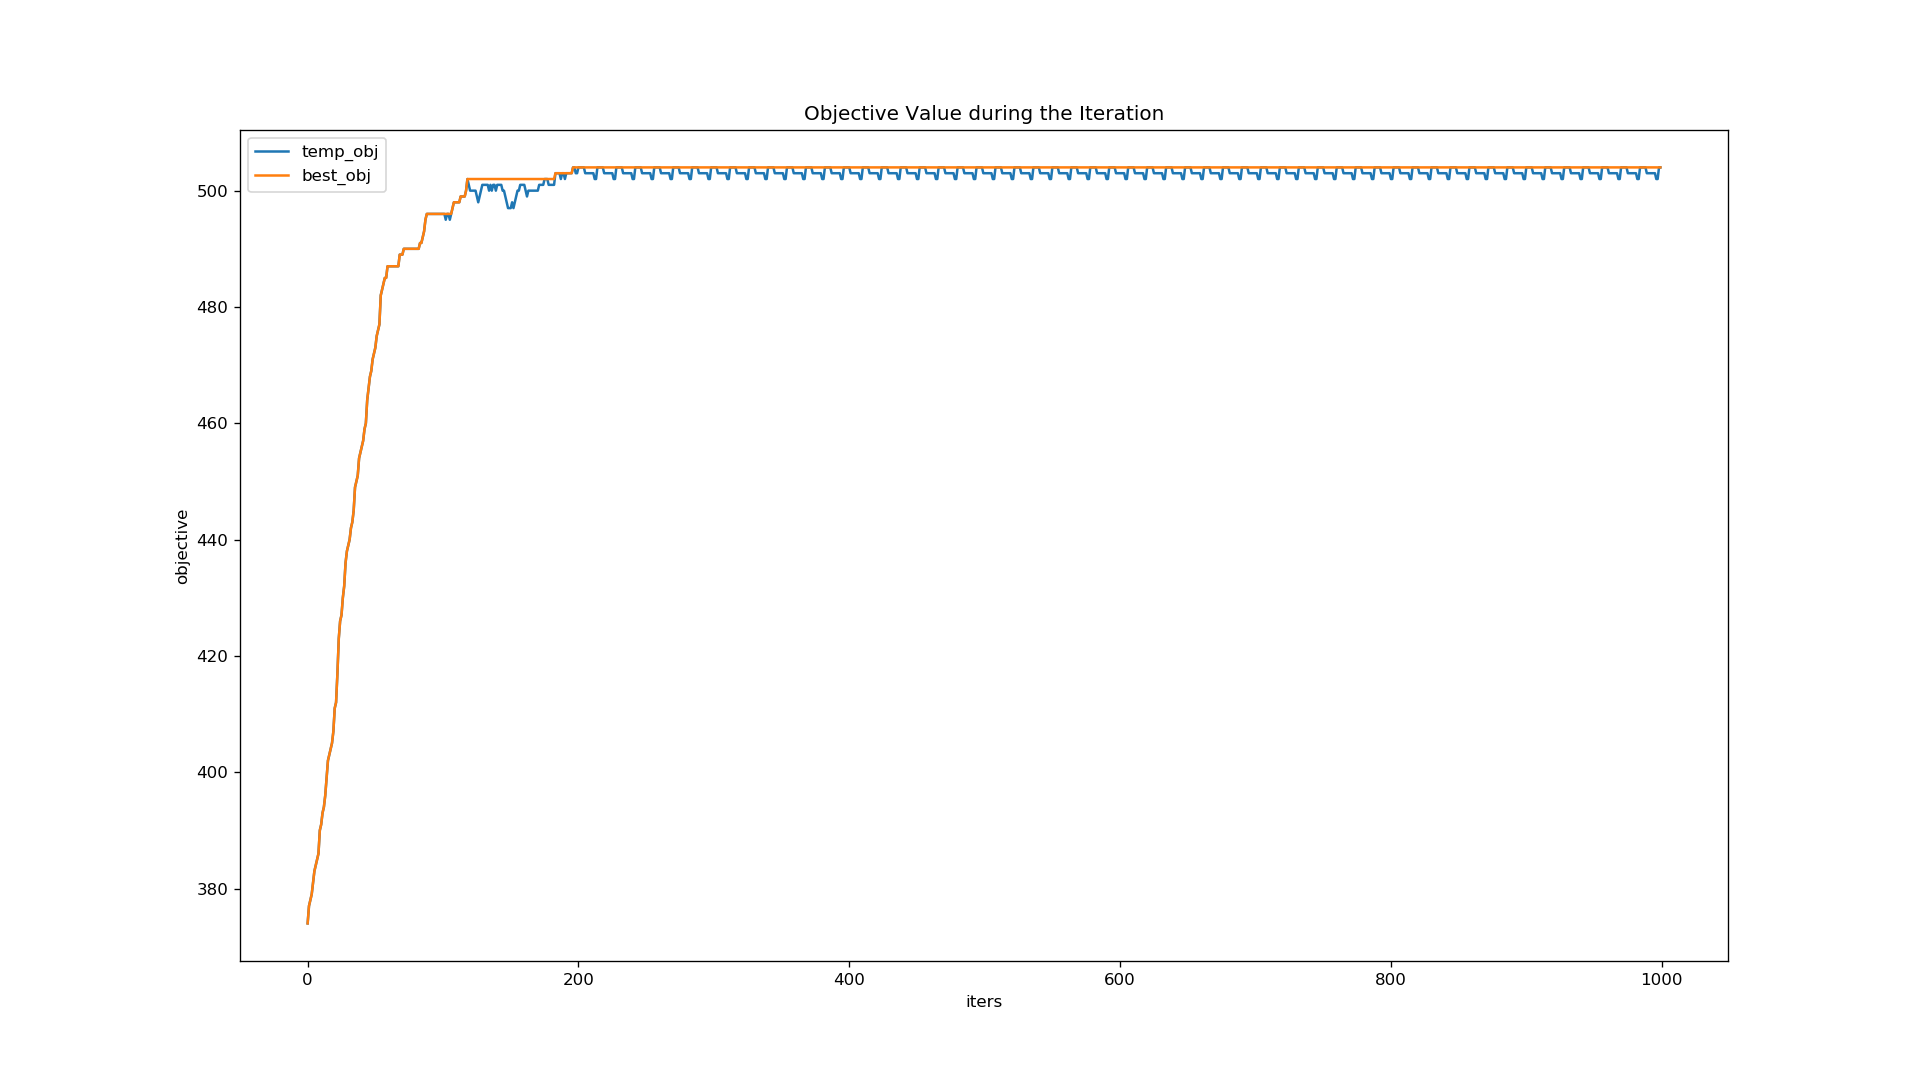
\includegraphics[width=\textwidth]{./image/tabu6.png}
        \caption{禁忌搜索算法迭代过程中目标值与最优目标值的变化}
    \end{figure}

    在前期,随机生成的初始解较差,目标值上升的很快,在破禁准则的作用下没有出现目标值下降的情况,随着迭代次数的增加,增速下降,目标值逐渐趋于收敛,出现跳出局部解的情况,最优目标值趋于固定值。最终,算法在局部最优解附近不断循环,最优目标值不再发生变化。

    接着,分别考察不同禁忌长度(5,10,20,30,40)下禁忌搜索算法迭代过程中目标值的变化:

    \begin{figure}[H]
        \centering
        \subfigure[目标值]{
            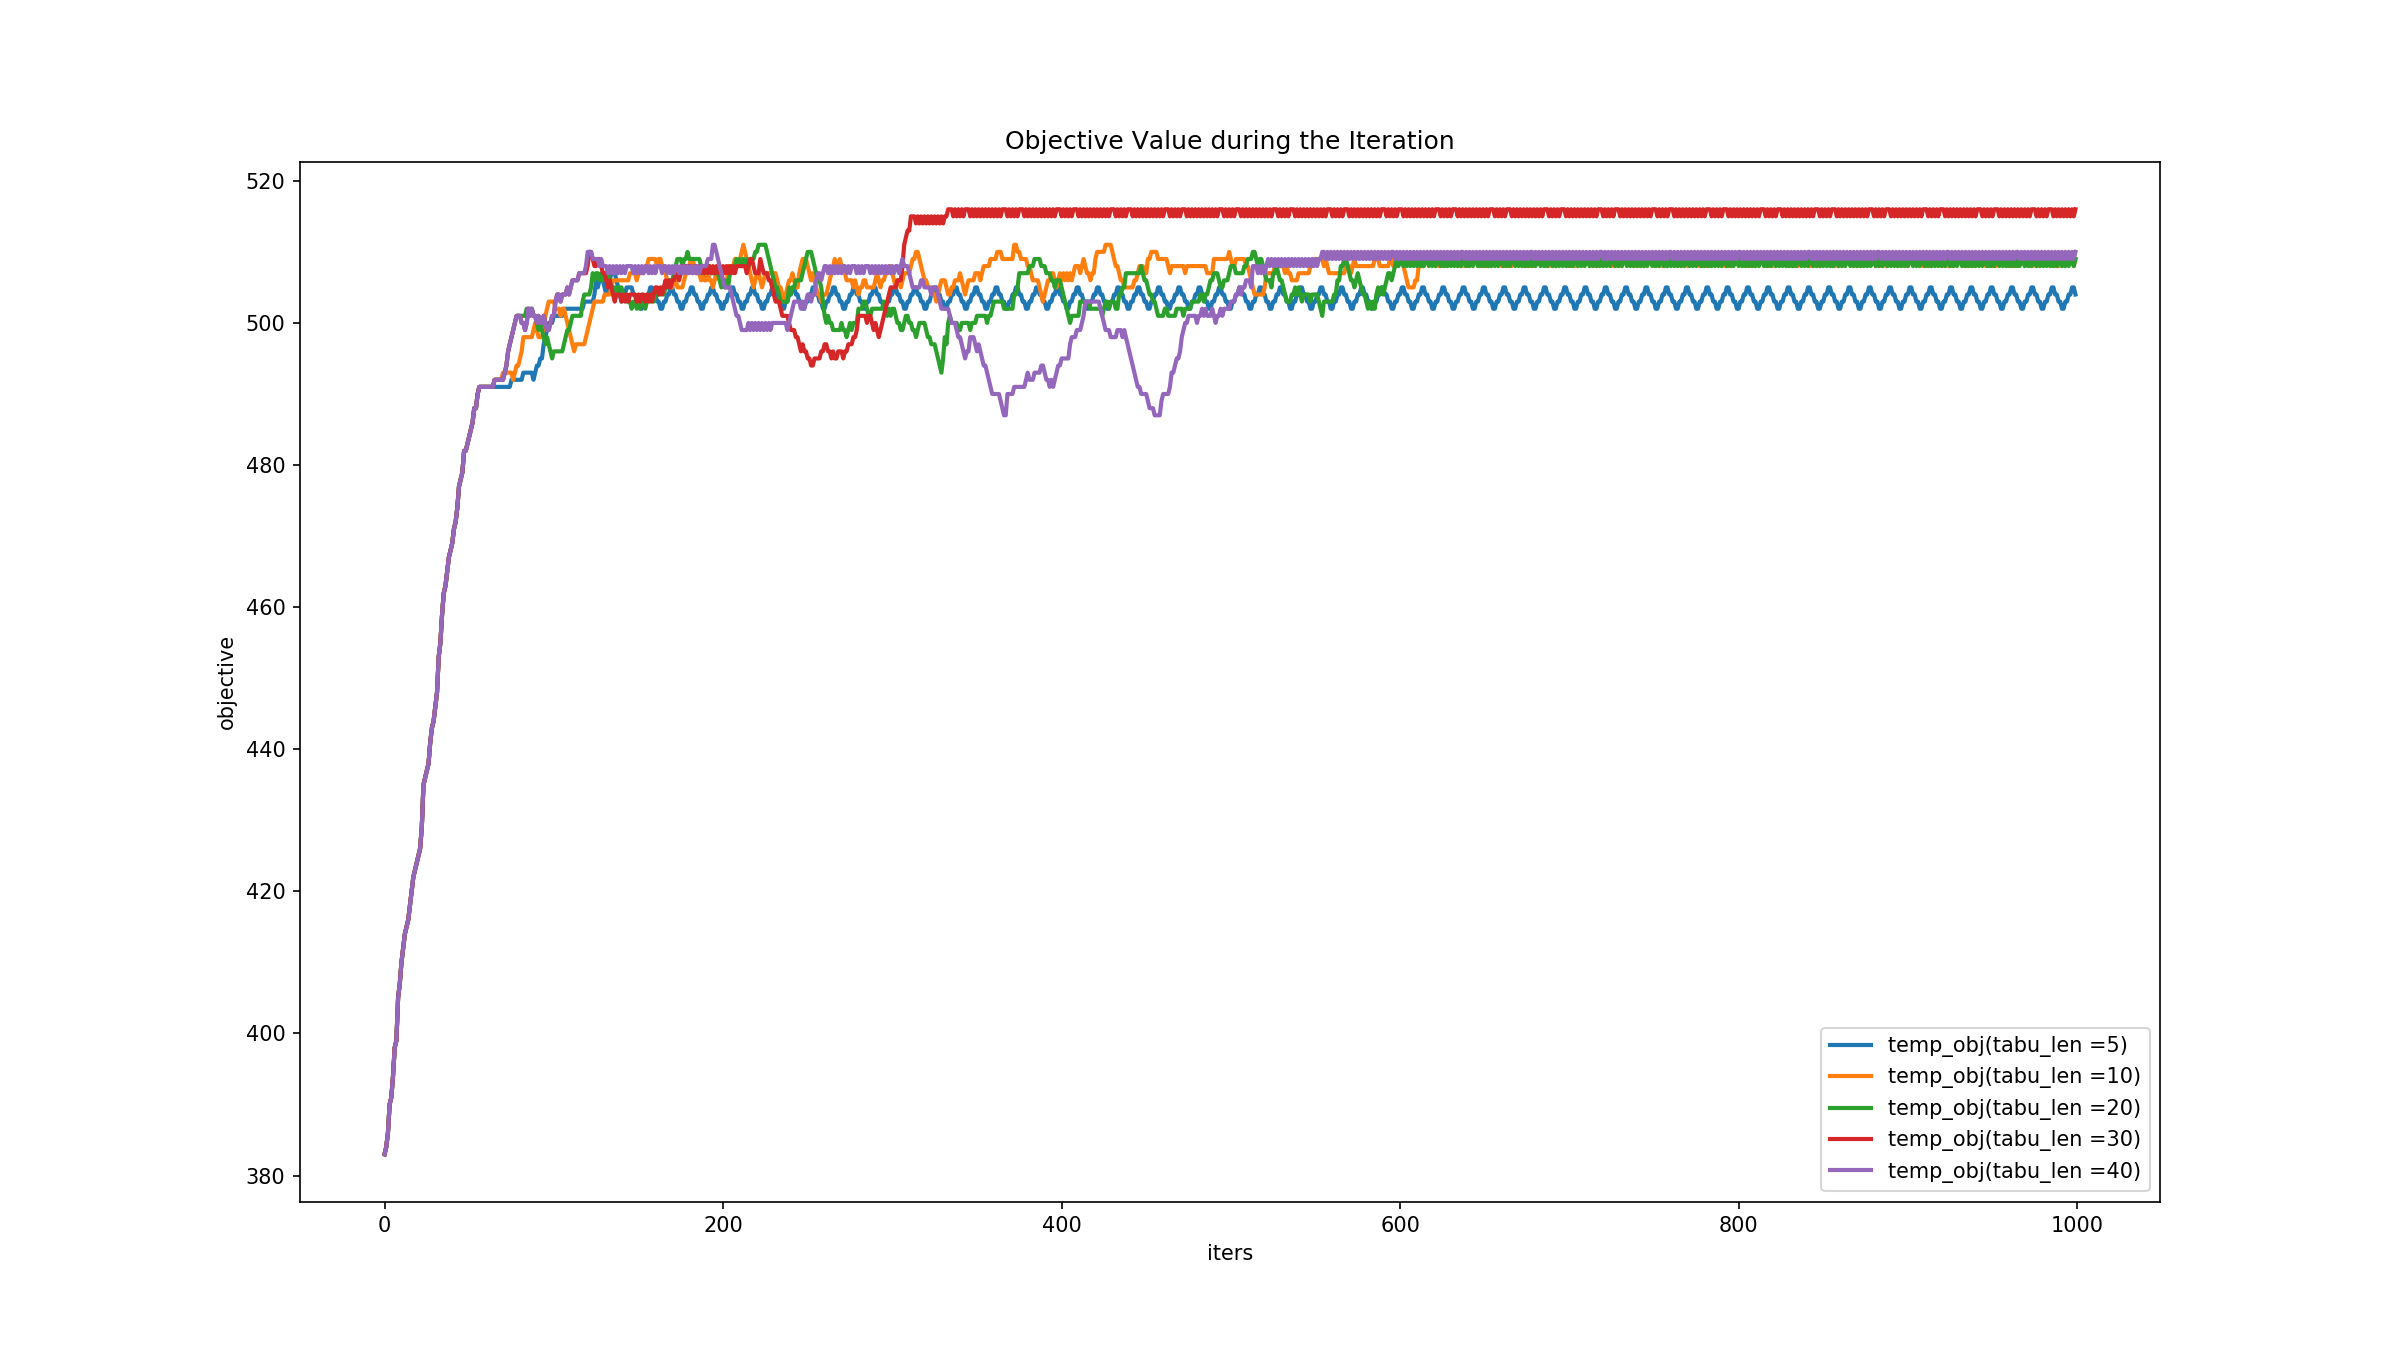
\includegraphics[width=\textwidth]{./image/tabu_all.png}
        }
        \quad
        \subfigure[最优目标值]{
            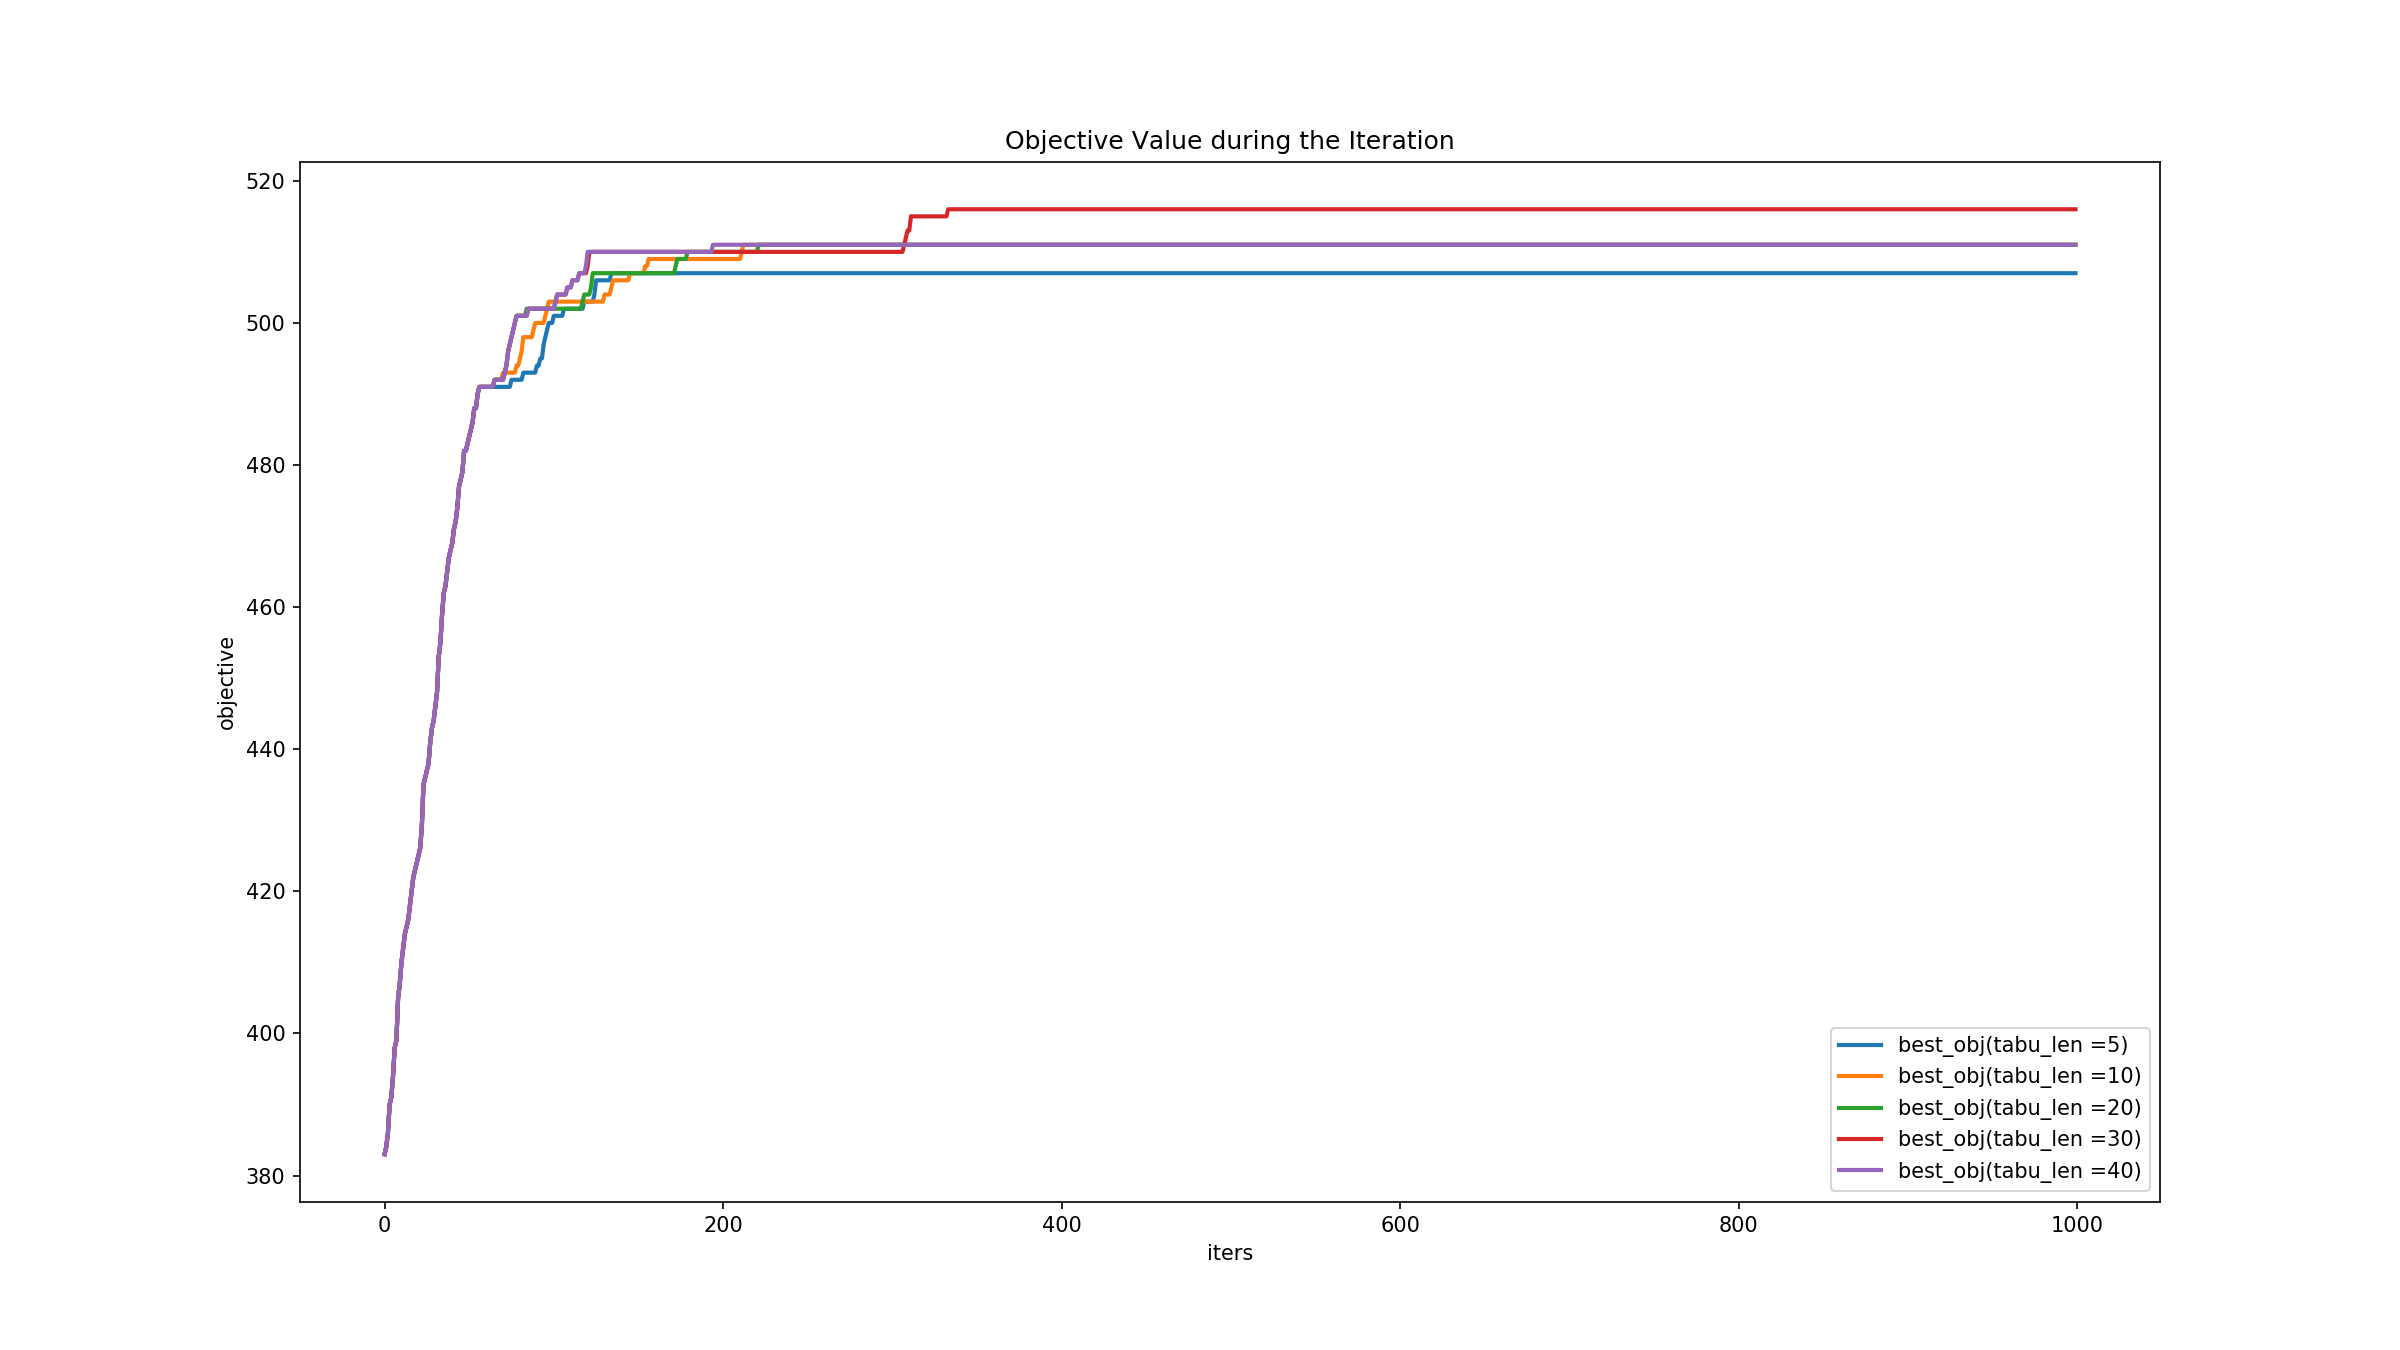
\includegraphics[width=\textwidth]{image/tabu_all_best.png}
        }
        \caption{不同禁忌长度下禁忌搜索算法迭代过程中目标值与最优目标值的变化}
    \end{figure}

    可以观察到,在前期,各禁忌长度下的迭代过程中目标值变化基本一致,目标值迅速上升。当迭代次数到达100次附近,目标值的变化随着禁忌长度的不同出现差异,禁忌长度较小者(禁忌长度=5)很快陷入局部最优解,目标值开始出现周期性特征。而随着禁忌长度的增加,在禁忌长度为10与20时,由于禁忌规则的存在,算法在第100-300次迭代过程中不断跳出局部最优解,解不断改进,使得最终的最优目标值相比禁忌长度为5时有了显著的提高。在禁忌长度达到20以后,尽管相比禁忌长度较小时得到的最优目标值有一定的改进,但由于算法每次迭代可选择的解减少,使得算法可能错过更优的解,因此,其最终的效果并不如禁忌长度为10,20的情况。
    
    根据5个给定的禁忌长度下的迭代图线,可以看出禁忌长度的设置不宜偏小,也不宜偏大,既要避免由于禁忌长度过小导致算法过早陷入局部最优,也要考虑禁忌长度过大导致效果的下降以及算法可能无法进行下去的情况。在该算例中,将禁忌长度设定在20附近,算法可以达到比较好的效果。

    \subsection{模拟退火算法}
    模拟退火算法中,设置冷却系数为0.99,初始温度为10000,冷却温度为1e-5,最大迭代次数为10000,得到结果如下:
    \begin{figure}[H]
        \centering
        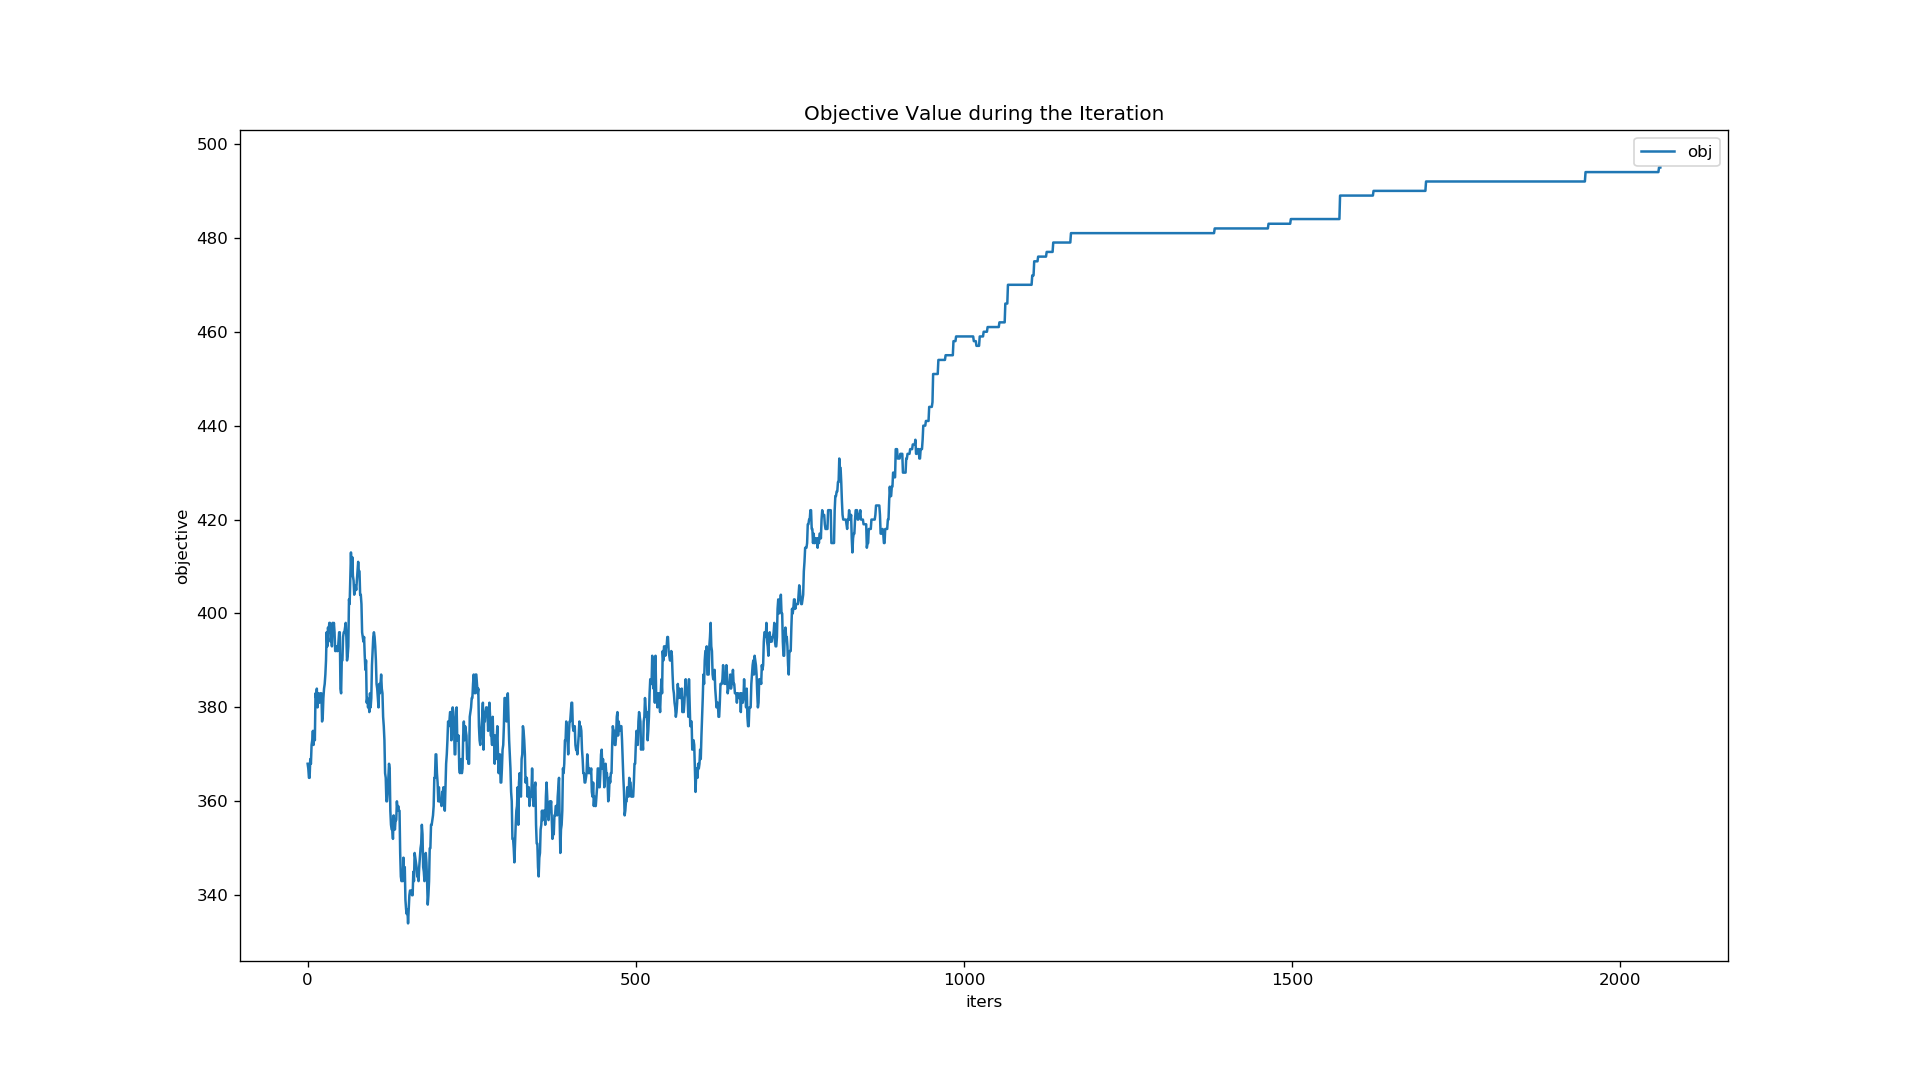
\includegraphics[width=\textwidth]{./image/sa.png}
        \caption{模拟退火算法迭代过程中目标值的变化}
    \end{figure}

    根据求解结果,可以看到模拟退火算法整体的目标值变化在前期呈现波动很大的现象,随着迭代次数的增加,波动越来越小,最终目标值呈现稳定上升的状态。这与算法原理一致,在运行前期,算法接受劣解的概率很大,因而目标值忽高忽低,随着迭代次数增加,接受劣解概率不断下降,最终只接受优解。

    \subsection{遗传算法}
    在遗传算法中,染色体交叉方式设定为2进制交叉,选择策略使用锦标赛算法,每一代群体数设置为30,变异概率设置为0.1。在前期测试时,最大迭代次数设置较小,图像在迭代即将终止时仍然保持上升趋势,因此,我们将最大迭代次数设置为400次,得到结果如下:
    \begin{figure}[H]
        \centering
        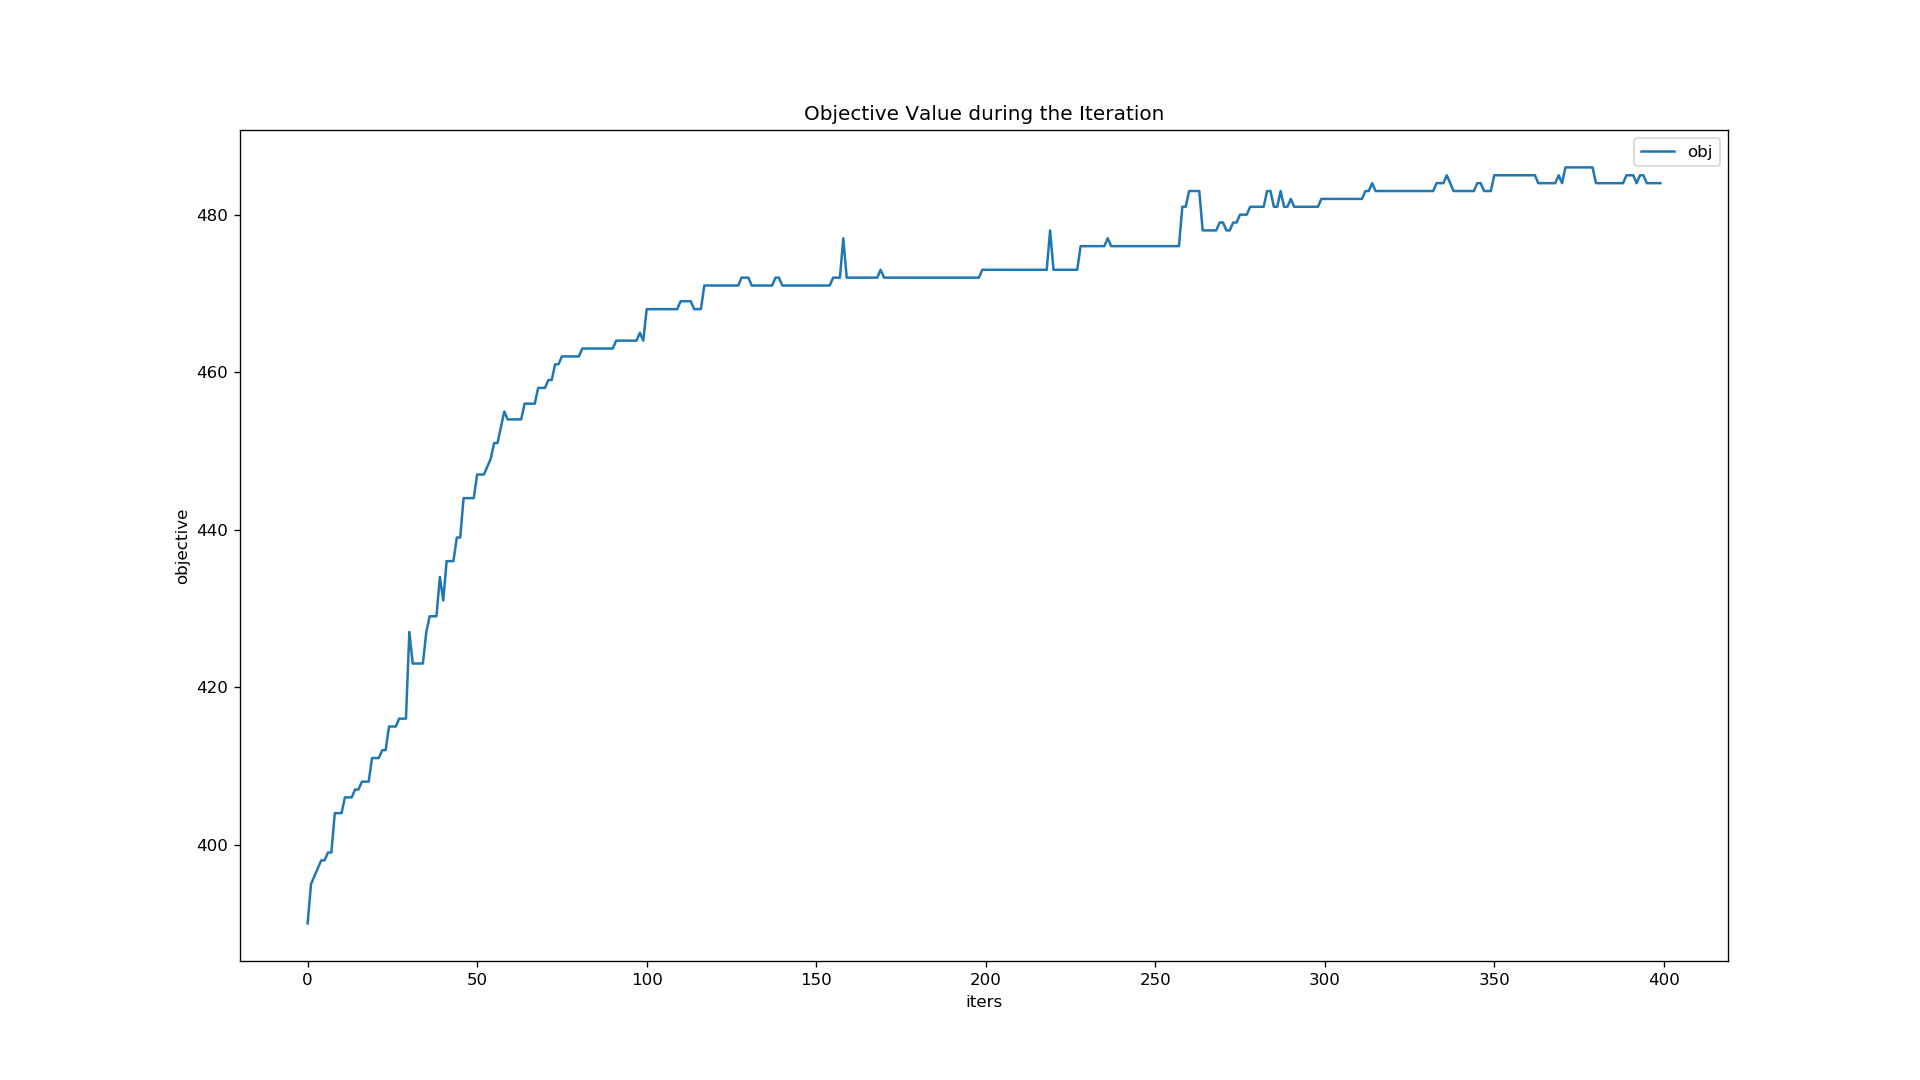
\includegraphics[width=\textwidth]{./image/ga.png}
        \caption{遗传算法每一代群体目标值的变化}
    \end{figure}

    相比前两种算法,遗传算法迭代过程中目标值增长的趋势相对稳定,每生成一批新的子代,目标值都有一定的增长,前期增长较快,迭代100期后增长渐渐减缓,之后每次解得到明显的改进所需迭代的期数越来越长,最终趋于稳定。

    在运算时间和运算效果上,遗传算法仅仅迭代400期就花费了约84s,相比之下,禁忌搜索算法与模拟退火算法迭代1000次的平均运算时间约为0.15s左右,收敛速度远快于遗传算法。同时,由于使用的算子相对简单,最终输出的解也不如前二者。

    \newpage
    \section{附录}
    \noindent
    read\_data.py,用于读取算例文件
    \begin{python}
    import numpy as np

    def read_data(file_name):
        """
        read data from txt
        :param file_name:
        :return: edge and nodes number p and edge number v
        """

        with open(file_name) as f:  # 自动关闭打开的资源语句
            data = f.readlines()  # 读取所有行
        _, p, v = data[0].replace('\n', '').split(' ')
        edges = np.zeros((int(p), int(p)))  # 构建表示节点是否连接的矩阵
        for i in data[1:]:
            if i == '\n':
                break  # 读取到最后一行单独为换行符时跳出循环
            line_data = i.split(' ')  # 划分每一行中的三个数据
            first, second = int(line_data[1]), int((line_data[2]).replace('\n', ''))  # 获取对应数据,如:e 5 1\n中的5与1
            first, second = min(first, second), max(first, second)  # 小者在前,大者在后,即行数取小,只记一次
            edges[first - 1, second - 1] = 1  # 有边设为1

        return edges, int(p), int(v)  # 返回节点边长矩阵以及节点数与边数
    \end{python}
    max\_cut\_instance.py,自定义最大割问题与问题解对应的类
    \begin{python}
from read_data import read_data
import random
import numpy as np
import time
class Problem_Instance:
    """
    the instance of a problem, consist of p,v and edge
    """
    p = 0
    v = 0
    edges = []

    def __init__(self, file_name):
        self.edges, self.p, self.v, = read_data(file_name)  # 运用读取的文件数据,初始化最大割问题实例


class Problem_solution:
    """
    a solution to the max-cut problem. '0' '1'  in the nodes which represents the in
    """
    nodes = []
    obj = 0
    updates = []  # 维护一个矩阵,储存了节点i从0-1的obj的变化值

    def __init__(self, instance):
        """
        init from a instance
        :param instance:
        """
        self.nodes = []
        self.obj = 0
        self.updates = []  # 维护一个矩阵,储存了节点i从0-1的obj的变化值
        random.seed(time.clock())
        for i in range(instance.p):
            self.nodes.append(random.randint(0, 1))  # 随机划分两个集合
            self.updates.append(0)  # 根据节点数初始化update矩阵
        for i in range(instance.p):
            delta = 0  # 变换节点所属集合后函数值变化量
            for j in range(instance.p):
                if instance.edges[min(i, j), max(i, j)] == 1:  # 两节点相连
                    if self.nodes[i] + self.nodes[j] == 1:  # 两节点不属于一个集合
                        delta += 1
                    else:
                        delta -= 1
            self.updates[i] = - delta
        self.get_obj(instance)

    def get_obj(self, instance):
        """
        对解进行更新
        :param instance:
        :return:
        """
        self.obj = 0
        for i in range(instance.p):
            for j in range(i, instance.p):
                if instance.edges[i, j] == 1 and self.nodes[i] != self.nodes[j]:
                    self.obj += 1  # 两节点相连且属于不同集合,计算当前所割总边数
        return self.obj

    def update(self, instance, i):  # 反转节点i后对解进行更新
        self.obj = self.obj + self.updates[i]
        for j in range(instance.p):
            if j == i:
                self.updates[j] = -self.updates[j]  # 原来的变负
            elif instance.edges[min(i, j), max(i, j)] == 1:  # 假如i,j有边连接
                if self.nodes[i] + self.nodes[j] == 1:
                    self.updates[j] -= 2  # 原来已在一个集合的-=2
                else:
                    self.updates[j] += 2  # 原来不在一个集合的+=2

    def __str__(self):
        return 'solution: {}\nobjective: {}'.format(self.nodes, self.obj)

    def __gt__(self, other):
        if self.obj >= other.obj:
            return True

    \end{python}
    tabu\_search.py,禁忌搜索算法
    \begin{python}
import max_cut_instance as m_instance
import local_search as ls
import record_process as rp

# 初始化禁忌长度、最大迭代次数
tabu_len_multi = 0.1
Max_iters = 10000

def tabu_search(solution, instance, tabu_len_multi=tabu_len_multi, Max_iters=Max_iters):
    """
    禁忌搜索算法,返回迭代相应次数后得到的最优解
    :param solution:初始解
    :param instance:算例
    :param tabu_len_multi:禁忌长度乘数(禁忌长度=[节点数*禁忌长度乘数])
    :param Max_iters:最大迭代次数
    :return:
    """
    tabu_len = int(instance.p * tabu_len_multi)  # 按节点数的百分比初始化禁忌长度
    tabu_list = [0 for i in range(instance.p)]  # 初始化禁忌表
    iter = 0  # 迭代次数
    best = solution.obj # 迭代当前最优值
    best_solution = solution
    record_data = "tabu_len: {}\n\n".format(tabu_len)

    while iter < Max_iters:
        solution_obj = solution.obj  # 当前解目标值
        local_temp = solution.updates[0]
        index = 0
        flag = 0
        record_data = record_data + "iteration: {}\n{}\nbest_obj: {}\n\n".format(iter,solution,best)
        print(solution.obj)

        for i in range(instance.p):
            temp = solution.updates[i]

            # 破禁准则
            if solution_obj + temp > best:
                index = i
                best = solution_obj + temp  # 破禁后更新最优值
                flag = 1
                break

            if tabu_list[i] != 0:  # 禁忌表数值非0时不予考虑
                continue
            elif temp > local_temp:
                local_temp = temp
                index = i

        solution = ls.flip(solution, index, instance)

        # 更新禁忌表
        tabu_list = [item - 1 if item > 0 else item for item in tabu_list]
        if flag == 0:  # 判断此次迭代是否为破禁后完成
            tabu_list[index] += tabu_len
        else:
            best_solution = solution  # 破禁后更新最优解

        iter += 1

    rp.record(record_data,'tabu{}'.format(tabu_len))
    return best_solution    
    \end{python}
    simulated\_annealing.py,模拟退火算法
    \begin{python}
import local_search as ls
import record_process as rp
import max_cut_instance as m_instance
import random as rd
import math

T = 10000  # 温度
T_min = pow(10,-5)  # 冷却温度
Max_iters = 10000  # 最大迭代次数
r = 0.99  # 降火


def E_evaluation(delta, T):
    """
    返回多大可能接受新解
    :param obj:
    :param new_obj:
    :return: 概率
    """
    if delta > 0:
        return 1
    else:
        return math.exp(delta / T)

def simulated_annealing(solution, instance, T=T, T_min=T_min, Max_iters=Max_iters, r=r):
    """
    模拟退火算法
    :param solution:
    :param instance:
    :param T:
    :param T_min:
    :param Max_iters:
    :param r:
    :return: 迭代对应次数所得解
    """
    iter = 0
    record_data = 'T {} T_min {} r {}\n\n'.format(T, T_min, r)

    while iter < Max_iters and T > T_min:
        record_data = record_data + "iteration: {}\n{}\n\n".format(iter, solution)
        i = rd.randint(0, instance.p - 1)
        delta = solution.updates[i]
        p = E_evaluation(delta, T)
        p_rd = rd.random()
        print(iter,solution.obj,T,p)

        if p_rd < p:
            solution = ls.flip(solution, i, instance)

        T = r * T
        iter += 1

    rp.record(record_data,"sa")
    return solution
    \end{python}
    genetic\_algorithm.py,遗传算法
    \begin{python}
import max_cut_instance as m_instance
import random as rd
import copy
from local_search import flip
import record_process as rp

T = 30  # 种群数量
max_iters = 400  # 最大迭代次数
alpha = 0.1  # 突变概率


def crossover(solution_A, solution_B, instance):
    """
    对两个解进行交叉,交叉方式为2进制交叉
    :param solution_A:
    :param solution_B:
    :return: 两个子代
    """
    j = rd.randint(0, instance.p - 1)
    mid = solution_A.nodes[j]
    solution_A.nodes[j] = solution_B.nodes[j]
    solution_B.nodes[j] = mid
    solution_A.get_obj(instance)
    solution_B.get_obj(instance)
    return solution_A, solution_B


def select(solutions, instance, T):
    """
    选择:从solutions 中获得下一代,方法使用锦标赛算法
    :param solutions: 种群
    :return: new_solutions 新种群
    """
    new_solutions = []
    for t in range(T):
        i = rd.randint(0, T - 2)
        j = rd.randint(i + 1, T - 1)  # 不断随机找子代
        solution = copy.deepcopy(max(solutions[i:j]))
        new_solutions.append(solution)
    return new_solutions


def mutation(solution, instance):
    """
    突变,单点变异,随机取反一位
    :param solution:原来的解
    :return: 随机反转以后的解
    """
    i = rd.randint(0, instance.p - 1)
    flip(solution, i, instance)
    return solution


def genetic_algorithm(instance, T=T, max_iters=max_iters, alpha=alpha):
    """
    对给定问题实例进行遗传算法
    :param instance: 问题实例
    :return: 返回一个solution,种群中最优解
    """
    solutions = []
    record_data = 'T {} alpha {}\n\n'.format(T, alpha)

    for i in range(T):  # 构造初始解
        solution = m_instance.Problem_solution(instance)
        solutions.append(solution)
    for i in range(max_iters):
        iter = i
        for j in range(T):  # 交叉
            i = rd.randint(0, T - 1)
            j = rd.randint(0, T - 1)  # 随机生成两个子代
            solutions[i], solutions[j] = crossover(solutions[i], solutions[j], instance=instance)
        for i in range(T):
            pd = rd.random()
            if pd < alpha:
                mutation(solutions[i], instance)  # 一定概率发生突变
        solutions = select(solutions, instance, T)  # 选择
        solution = max(solutions)
        record_data = record_data + "generation: {}\n{}\n\n".format(iter, solution)
        print(solution.obj)
    solution = max(solutions)
    rp.record(record_data, "ga")
    return solution
    \end{python}
\end{document}